\documentclass{article}

% if you need to pass options to natbib, use, e.g.:
%     \PassOptionsToPackage{numbers, compress}{natbib}
% before loading neurips_2026

% The authors should use one of these tracks.
% Before accepting by the NeurIPS conference, select one of the options below.
% 0. "default" for submission

%\PassOptionsToPackage{numbers, compress}{natbib}

\usepackage{neurips_2026}
% the "default" option is equal to the "main" option, which is used for the Main Track with double-blind reviewing.
% 1. "main" option is used for the Main Track
%  \usepackage[main]{neurips_2026}
% 2. "position" option is used for the Position Paper Track
%  \usepackage[position]{neurips_2026}
% 3. "eandd" option is used for the Evaluations & Datasets Track
 % \usepackage[eandd]{neurips_2026}
% 4. "creativeai" option is used for the Creative AI Track
%  \usepackage[creativeai]{neurips_2026}
% 5. "sglblindworkshop" option is used for the Workshop with single-blind reviewing
 % \usepackage[sglblindworkshop]{neurips_2026}
% 6. "dblblindworkshop" option is used for the Workshop with double-blind reviewing
%  \usepackage[dblblindworkshop]{neurips_2026}
% 7. "education" option is used for the Education Track
%  \usepackage[education]{neurips_2026}


% After being accepted, the authors should add "final" behind the track to compile a camera-ready version.
% 1. Main Track
 % \usepackage[main, final]{neurips_2026}
% 2. Position Paper Track
%  \usepackage[position, final]{neurips_2026}
% 3. Evaluations & Datasets Track
 % \usepackage[eandd, final]{neurips_2026}
% 4. Creative AI Track
%  \usepackage[creativeai, final]{neurips_2026}
% 5. Workshop with single-blind reviewing
%  \usepackage[sglblindworkshop, final]{neurips_2026}
% 6. Workshop with double-blind reviewing
%  \usepackage[dblblindworkshop, final]{neurips_2026}
% Note. For the workshop paper template, both \title{} and \workshoptitle{} are required, with the former indicating the paper title shown in the title and the latter indicating the workshop title displayed in the footnote.
% For workshops (5., 6.), the authors should add the name of the workshop, "\workshoptitle" command is used to set the workshop title.
% \workshoptitle{WORKSHOP TITLE}
% 7. Education Track
% \usepackage[education, final]{neurips_2026}

% "preprint" option is used for arXiv or other preprint submissions
 % \usepackage[preprint]{neurips_2026}

% to avoid loading the natbib package, add option nonatbib:
%    \usepackage[nonatbib]{neurips_2026}

\usepackage[utf8]{inputenc} % allow utf-8 input
\usepackage[T1]{fontenc}    % use 8-bit T1 fonts
\usepackage{hyperref}       % hyperlinks
\usepackage{url}            % simple URL typesetting
\usepackage{booktabs}       % professional-quality tables
\usepackage{amsfonts}       % blackboard math symbols
\usepackage{nicefrac}       % compact symbols for 1/2, etc.
\usepackage{microtype}      % microtypography
\usepackage{xcolor}         % colors
\usepackage{graphicx}
\usepackage{subcaption}
\usepackage{float}

% Note. For the workshop paper template, both \title{} and \workshoptitle{} are required, with the former indicating the paper title shown in the title and the latter indicating the workshop title displayed in the footnote. 
\title{In-Context-Learning of Black-Scholes in Transformers \\ \vspace{0.5 em}\small{Subtitle?}}


% The \author macro works with any number of authors. There are two commands
% used to separate the names and addresses of multiple authors: \And and \AND.
%
% Using \And between authors leaves it to LaTeX to determine where to break the
% lines. Using \AND forces a line break at that point. So, if LaTeX puts 3 of 4
% authors names on the first line, and the last on the second line, try using
% \AND instead of \And before the third author name.


\author{%
  David S.~Hippocampus\thanks{Use footnote for providing further information
    about author (webpage, alternative address)---\emph{not} for acknowledging
    funding agencies.} \\
  Department of Computer Science\\
  Cranberry-Lemon University\\
  Pittsburgh, PA 15213 \\
  \texttt{hippo@cs.cranberry-lemon.edu} \\
  % examples of more authors
  % \And
  % Coauthor \\
  % Affiliation \\
  % Address \\
  % \texttt{email} \\
  % \AND
  % Coauthor \\
  % Affiliation \\
  % Address \\
  % \texttt{email} \\
  % \And
  % Coauthor \\
  % Affiliation \\
  % Address \\
  % \texttt{email} \\
  % \And
  % Coauthor \\
  % Affiliation \\
  % Address \\
  % \texttt{email} \\
}


\begin{document}


\maketitle

\begin{abstract}
    \citet{garg2022what} show that transformers can learn several function classes in
    context. We review this work and reproduce some of its results for linear functions,
    where our own transformer matches the error of least squares. We then apply
    in-context learning to Black--Scholes pricing of European options. Each prompt
    contains priced options on one underlying (asset) whose volatility is unknown and either flat
    or follows a smile. After a single example, the transformer improves far on the
    no-context prior mean. With few examples it outperforms correctly specified
    calibration on smile volatility, and on noisy prices it approaches the noise floor.
    However, it degrades for strikes far outside the training range, suggesting that it
    has learned an approximation that holds within the training distribution rather than
    the pricing formula itself.
\end{abstract}

\section{Introduction}
In-Context Learning (ICL) refers to the ability of a machine learning model to solve a task conditioned on examples of input-output pairs given in the prompt at inference time, without any updates to the model weights. So the "learning" (of weights $w$ for linear $f(x)=w^Tx$ for example) happens in the activations during the forward pass, while the weights of the model only encode the optimization algorithm.

An intuitive example motivating how tranformers can encode optimization procedures, such as gradient descent is presented by \cite{vonOswald2023Transformers}, restated here in a simpler and less rigourus way. 

Consider a least squares problem with training data $\{(x_i, y_i)\}_{i=1}^N$ where $y(x)=w^Tx$, with objective function
\begin{equation}
    L(w)=\frac{1}{2N}\sum_{i=1}^N ||w^Tx_i-y_i||^2.
\end{equation}

Consider the weight update in one step of gradient descent with step size $\eta$
\begin{equation}
    \Delta w
= -\eta \nabla_w L(w)
= -\eta \sum_{i=1}^{N} (w^T x_i - y_i)x_i.
\end{equation}

Also assume initial weights $w_0=0$, then

\begin{equation}
    w_1 = w_0 +\Delta w_0 
= \eta \sum_{i=1}^{N} y_i x_i.
\end{equation}

The prediction for the query based on the approximation of $w$ after a single step of gradient descent is
\begin{equation}
    \hat{y_q} = w_1^Tx_q = \eta \sum_{i=1}^{N} y_i x_i^Tx_q.
\end{equation}





\section{A review of \citet{garg2022what}}
% (a) Recap of the main algorithm, its mathematical formulation, and the main thesis of the paper, which you may be questioned on

In this section we review the theory and methods used by \cite{garg2022what}.

\paragraph{Hypothesis.} The hypothesis of the paper is that transformers trained on
specific families of functions, including linear functions, sparse linear functions,
two-layer neural networks, and decision trees, can encode non-trivial learning algorithms
within a single forward pass. Therefore, given in-context examples from a new function
drawn from such a function class, never seen during training, transformers can predict the
function's value at a new query input. ICL is hard to study in LLMs, so the paper invents a
controlled setting to study the phenomenon in transformers only. Concretely for linear
functions, given a set of pairs $\{(x_i, f(x_i))\}_{i=1}^k$ from $f(x)=w^\top x$, a
transformer encodes an algorithm which lets it infer the weights $w$ to predict
$f(x_{k+1})$, resembling least squares. Since every prompt uses a new $w$, memorising a
single function cannot work; the model has to learn how to infer $w$ from the examples.

\paragraph{Formulation.} Let $D_\mathcal{X}$ be a distribution over inputs and
  $D_\mathcal{F}$ a distribution over functions in $\mathcal{F}$. A prompt is a sequence of
  pairs $(x_i, f(x_i))$ followed by a query:
  \begin{equation}
    P =(x_1, f(x_1), \dots, x_k, f(x_k), x_{\text{query}}),
    \label{prompt}
  \end{equation}
with $x_i, x_{\text{query}} \sim D_\mathcal{X}$ i.i.d.\ and $f \sim D_\mathcal{F}$.
A model $M$ \emph{in-context learns} $\mathcal{F}$ up to $\epsilon$ if for some loss
function $\ell$
\begin{equation}
\mathbb{E}_P\!\left[\ell\big(M(P), f(x_{\text{query}})\big)\right] \le \epsilon.
\end{equation}

\paragraph{Training.} A decoder-only GPT-2 style transformer $M_\theta$
(12 layers, 8 heads, 256-dimensional embeddings, 9.5M parameters) is trained
from scratch without any text or pre-trained language model. For
each training step, a function $f$ from the function class and inputs $x_i$ are sampled,
and the model is trained to predict $f(x_{i+1})$ from every prompt prefix
$P^i = (x_1, f(x_1), \dots, x_i, f(x_i), x_{i+1})$, with the objective to minimize
\begin{equation}
\mathbb{E}_P\!\left[\frac{1}{k+1}\sum_{i=0}^{k}
\ell\big(M_\theta(P^i), f(x_{i+1})\big)\right].
\end{equation}

For linear functions, which we study further in this report because of their simplicity
and the particularly interesting ICL behavior, $x_i \sim \mathcal{N}(0, I_d)$,
$f(x)=w^\top x$ with $w \sim \mathcal{N}(0, I_d)$, and $d=20$. Training uses Adam,
500k steps with batch size 64 and a curriculum that gradually increases the input
dimension and prompt length, which significantly speeds up training.

\paragraph{Evaluation.} The transformer trained for ICL is evaluated with respect to the
normalized (by dimension $d$) squared error
\begin{equation}
  \frac{1}{d}(M(P)-f(x_{\text{query}}))^2
  \label{error}
\end{equation}
on prompts $P$ according to \eqref{prompt}, where $k$ is the number of in-context
examples. Its performance in terms of error \eqref{error} is compared to classical
alternatives as a function of the number of in-context examples.

For linear functions, the transformer is compared to minimum-norm least squares, which is
optimal for this noiseless problem, an averaging estimator
$\hat{w}=\frac1k\sum_i x_i y_i$, and 3-nearest neighbours.

\paragraph{Results.}
For linear functions, the trained transformer's error tracks that of least squares for
every number of in-context examples, and is far better than averaging or nearest
neighbours. Performance degrades gracefully under skewed input covariance, a
low-dimensional input subspace, and mismatches between the in-context examples and the
query. It is less robust to rescaling the inputs. The transformer also handles noisy
labels and even reproduces the double descent curve of least squares.

Transformers also learn (i) sparse linear functions, matching Lasso,
(ii) two-layer ReLU networks, matching a network trained by Adam on the context, and
(iii) depth-4 decision trees, outperforming greedy tree learning and XGBoost.

Larger models give lower error and are more robust to distribution shift, and curriculum
learning speeds up training drastically, especially in higher dimensions.
\section{Reproduction of ICL of linear functions}
% (b) your reproduction, with a short log of what the paper left unspecified and what you had to guess

\subsection{Setup}
We train our own transformer from scratch on an NVIDIA A100 via Modal, using the same
model, optimiser, curriculum and
number of training steps as \cite{garg2022what}. As in the paper, we evaluate on 1280
prompts with 90\% bootstrap confidence intervals.

The paper does not state how many training runs its main results are based on, and the
authors released one checkpoint per task. We train a single run. Since neither their code
nor ours fixes a random seed, our error bars reflect variation over evaluation prompts
only. Otherwise we differ only in software (Python 3.10 instead of 3.8) and hardware
(A100 instead of RTX 3090), which change neither the model nor the training procedure.

\subsection{Results}

\paragraph{Clean labels.}
The transformer outperforms 3-NN and averaging, and its error closely tracks that of
minimum-norm least squares (Figure~\ref{fig:linear}, Table~\ref{tab:linear-repro}),
including the drop to zero error at $k \geq 20$, where the 20-dimensional problem is
fully determined and least squares has a unique solution.

\paragraph{Noisy labels.}
With noisy labels, the transformer still outperforms 3-NN and averaging, and reproduces
the double descent curve (Figure~\ref{fig:noisy}). For minimum-norm least squares, this
curve appears when test error is plotted against the number of noisy training samples
$n$ for a fixed number of features $p$ (here $n = k$, $p = d = 20$). For $n < p$, the
system is underdetermined. Among the infinitely many exact fits, the minimum-norm
solution keeps the weights small and spreads the noise over many directions, so
predictions on new data stay reasonable. At $n = p$, the fit is unique and must pass
through every noisy label. This requires large weights, which turn label noise into large
test errors, so the error peaks. For $n > p$, the problem is overdetermined and the noise
averages out as $n$ grows. Interestingly, the transformer handles the peak at $n = p$
better than minimum-norm least squares. This possibly suggests some kind of
regularisation of the in-context learned weights that keeps them from taking extreme
values.

\paragraph{Comparison with the released checkpoints.}
Our transformer performs like the checkpoints released by \cite{garg2022what}, up to
random variation; see Appendix~\ref{app:reproduction}.

\begin{figure}[H]
\centering
\begin{subfigure}[t]{0.38\textwidth}
  \centering
  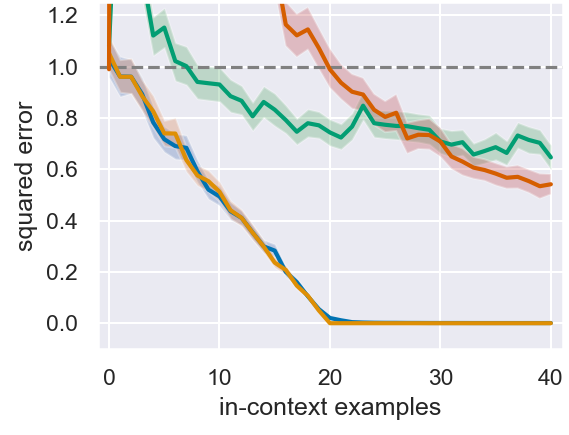
\includegraphics[width=\linewidth]{figures/standard_repr_cropped.png}
  \caption{Clean labels}
  \label{fig:linear}
\end{subfigure}\hfill
\begin{subfigure}[t]{0.58\textwidth}
  \centering
  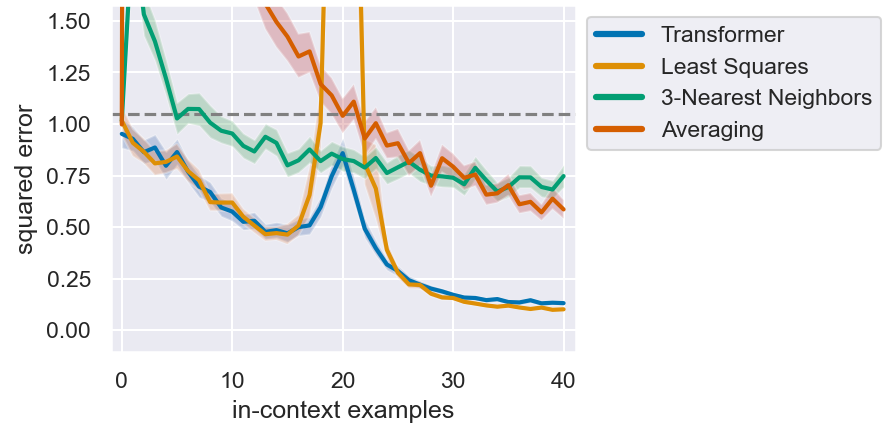
\includegraphics[width=\linewidth]{figures/noisyLR_repr_cropped.png}
  \caption{Noisy labels}
  \label{fig:noisy}
\end{subfigure}
\caption{ICL performance of our trained transformer on linear functions.}
\label{fig:repr}
\end{figure}
\section{In-Context-Learning of Black-Scholes}

As an extension of the work presented in \cite{garg2022what}, we intent to test the learning-to-learn and predictive abilities of transformer on a real world financial application: the European Option Market. 

\subsection{Introduction to Black-Scholes}

Relevant financial glossary is defined in \ref{app:glossary}.

Consider a stock that trades at \emph{spot price} $S$ today. A \emph{call option} on this stock
gives its holder the right, but not the obligation, to buy the stock at a fixed
\emph{strike} price $K$ at a fixed \emph{maturity} $T$ years from now.
This call option has a price $C$ today, which is usually much smaller than the stock price, and depends strongly on how much the stock's \emph{volatility} $\sigma$. A worked example is presented in appendix \ref{app:call_price}.


Price $S$, strike $K$ and maturity $T$ and are written in the contract and observable, but the volatility $\sigma$ is not. In practice it is inferred from the prices of other options
on the same stock. This is precisely an in-context
learning problem: given example (option, price) pairs on one stock, predict the price of
another option on that stock.

The Black-Scholes model makes this relationship precise. We define a new family of
functions, Black-Scholes functions, as
\begin{equation}
  \frac{C}{S} = \Phi(d_1) - e^{m - rT}\,\Phi(d_2), \qquad
  d_1 = \frac{-m + \left(r + \tfrac{1}{2}\sigma^2\right)T}{\sigma\sqrt{T}}, \qquad
  d_2 = d_1 - \sigma\sqrt{T},
  \label{bs}
\end{equation}
with $C, S, K, T$ as previously, $m = \ln(K/S)$ is the log-moneyness, $r = 0.02$ the risk-free rate (known), and $\Phi$ the standard normal CDF.
The function is non-linear but low dimensional: two inputs/features $(m, T)$ and one unknown parameters $\sigma$.

The unknown volatility $\sigma$ should be learned by the transformer from in-context
examples, and used to infer the standardised call price $C/S$ of a new option on the same asset.
We consider two variations of the problem: (i) \emph{flat volatility}, each
prompt has a constant volatility sampled  $\sigma \sim U[0.1, 0.5]$ per prompt. (ii)
\emph{smile volatility},
\begin{equation}
  \sigma(m) = \max\{\sigma_0 + b\,m + c\,m^2,\ 0.05\}, \quad
  \sigma_0 \sim U[0.15, 0.4],\ b \sim U[-0.4, 0],\ c \sim U[0, 1].
\end{equation}
The latter takes into account that implied volatility observed in markets varies with strike (skew $b$ and curvature $c$), and is therefore a more
realistic model. Consequently the transformer must effectively infer three parameters from the context instead of one, as in the flat volatility setting.

\subsection{Training and evaluation setup}

We use the same training setup as described in \cite{garg2022what}, except that the
curriculum only increases the number of examples, since $d = 2$ is fixed. The prompt is
\begin{equation}
P_{BS} = \big(x_1, f_\theta(x_1), \dots, x_k, f_\theta(x_k), x_{\text{query}}\big),
\qquad x_i, x_{\text{query}} \sim \mathcal{N}(0, I_2),
\end{equation}
where the hidden volatility parameters $\theta$, $\sigma$ for flat and $(\sigma_0, b, c)$
for smile volatility, are drawn once per prompt. As in \cite{garg2022what}, the inputs are
Gaussian; they are mapped to option features $m(x)$ and $T(x)$ by
Table~\ref{tab:bs-inputs}.

\begin{table}[h]
\caption{Input encoding for the Black--Scholes tasks ($d = 2$).}
\label{tab:bs-inputs}
\centering
\small
\begin{tabular}{lll}
\toprule
Input & Option feature & Meaning \\
\midrule
$x^{(1)}$ & log-moneyness $m = 0.2\,x^{(1)}$
  & strike relative to today's price, $m = \ln(K/S)$ \\
$x^{(2)}$ & maturity $T = 0.1 + 1.9\,\Phi(x^{(2)})$
  & years until expiry, $T \in [0.1, 2]$ \\
\bottomrule
\end{tabular}
\end{table}

The target $f_\theta(x)$ is the price $C/S$ from equation \eqref{bs}, evaluated at
$m(x)$, $T(x)$ and $\sigma = \sigma_\theta(m(x))$, and standardised by its mean and
standard deviation under the prior.\footnote{We standardise for two reasons. First,
it gives an interpretable error: predicting the mean gives error $\approx 1$, so errors
read as the fraction of price variance left unexplained. This plays the role of the
normalisation by $d$ in \eqref{error}, which we therefore do not apply. Second, raw
prices are small ($C/S \approx 0.14 \pm 0.10$) compared with the standard normal
inputs, and standardising puts inputs and targets on the same scale.}
The mean and standard deviation are fixed constants computed once by Monte Carlo
($\mu = 0.145$, $s = 0.102$ for flat and $\mu = 0.141$, $s = 0.106$ for smile volatility):
\begin{equation}
y = \frac{C/S - \mu}{s}.
\end{equation}
Since the transformation is fixed and invertible, $C/S = s\,y + \mu$, and all baselines
predict on the same scale, it does not change the task.

We compare the squared error of the transformer's prediction, without the normalisation
by $d$, to a baseline calibration method, which fits the volatility parameters to the
in-context examples by least squares and prices the query with the fitted parameters,
\begin{equation}
\hat\theta = \arg\min_{\theta'} \sum_{i=1}^{k} \big(f_{\theta'}(x_i) - y_i\big)^2,
\qquad \hat y_{\text{query}} = f_{\hat\theta}(x_{\text{query}}),
\end{equation}
where $y_i = f_\theta(x_i)$ are the prices given in the prompt. This mirrors how
practitioners calibrate implied volatility. On clean prices, once the examples determine
$\theta$ uniquely ($k \geq 1$ for flat, typically $k \geq 3$ for smile volatility), the true
parameters fit exactly and calibration recovers them, so its error is zero in principle.
With fewer examples than parameters, many volatility curves fit the examples exactly and
least squares returns an arbitrary one, so calibration is not optimal in that regime. In
practice, the minimisation is solved by a grid search followed by five rounds of local
refinement.

For the smile volatility task we run calibration both with the smile model that generated
the data and with a misspecified flat model, to test whether the transformer uses the
smile. The flat model acts as a stand-in for a lazy strategy: a transformer could get a
decent error on the smile task by estimating one average volatility from the examples and
ignoring how $\sigma$ changes with strike. If it did that, its error would flatten out at
the level of flat calibration.

Since the pricing formula is the same in every prompt, a transformer could learn an
average price surface in its weights without using the context. We therefore also
report a no-context baseline, the prior-mean price
$\hat y_{\text{query}} = \mathbb{E}_\theta\big[f_\theta(x_{\text{query}})\big]$. Only error
below this baseline is evidence of in-context learning of $\sigma$.

We evaluate the transformer's ability to in-context learn $\sigma$ and infer option prices
under clean and noisy prices. In the noisy setting, $\varepsilon \sim \mathcal{N}(0, \tau^2)$
with $\tau = 0.05$ is added to the standardised prices of both the examples and the query,
simulating bid--ask noise (the analogue of noisy linear regression in \cite{garg2022what}).
Since the query's noise cannot be predicted, no method can achieve an error below
$\tau^2 = 0.0025$. The model is trained on clean prices only.

Finally, we test robustness to a distribution shift without retraining, by scaling the
moneyness input $x^{(1)}$ of all examples and the query by 2 and 3, the analogue of input
scaling in \cite{garg2022what}. Since $m = 0.2\,x^{(1)}$ with $x^{(1)} \sim \mathcal{N}(0, 1)$, only 5\% of training options
have $|m| > 0.4$. Under scaling by 3, half of all options lie in this region, and 5\% have
$|m| > 1.2$, where the model has practically never been trained.

\subsection{Results}

\paragraph{Flat and smile volatility.}
\textbf{[How to read the numbers: what error 1 means, and why the prior mean, not 1,
is the bar for in-context learning.]}
In both tasks the transformer starts at the prior mean without examples and falls far
below it after a single example (Table~\ref{tab:bs-results}). With flat volatility it
stays above calibration for all $k$, and both level off after a few examples, the
transformer about an order of magnitude higher. With smile volatility the transformer
goes far below misspecified flat calibration, which levels off early. Compared with
smile calibration, it has lower error up to $k \approx 18$, the two are comparable up to
$k \approx 25$, and calibration is lower beyond (Figure~\ref{fig:bs-smile-noise}, left).
\textbf{[Interpretation: what $k=0$ vs.\ $k=1$ shows; why both level off above zero;
what the gap to flat calibration shows; why the transformer beats smile calibration,
and why only up to $k \approx 18$.]}

\begin{table}[h]
\caption{\textbf{[YOUR caption: what the table shows + key take-away]}}
\label{tab:bs-results}
\centering
\small
\begin{tabular}{llcccc}
\toprule
Task & Method & $k=0$ & $k=1$ & $k=3$ & $k=40$ \\
\midrule
Flat & Transformer & $0.146$ & $3.4\cdot10^{-3}$ & $7.2\cdot10^{-5}$ & $1.8\cdot10^{-5}$ \\
 & Calibration & $0.144$ & $1.1\cdot10^{-4}$ & $1.2\cdot10^{-6}$ & $1.2\cdot10^{-6}$ \\
 & Prior mean (no context) & $0.157$ & $0.156$ & $0.149$ & $0.149$ \\
\midrule
Smile & Transformer & $0.061$ & $\mathbf{1.1\cdot10^{-2}}$ & $\mathbf{1.2\cdot10^{-3}}$ & $1.5\cdot10^{-5}$ \\
 & Calibration (smile) & $0.060$ & $2.1\cdot10^{-2}$ & $3.1\cdot10^{-3}$ & $7.1\cdot10^{-6}$ \\
 & Calibration (flat) & $0.059$ & $4.5\cdot10^{-2}$ & $2.4\cdot10^{-2}$ & $1.5\cdot10^{-2}$ \\
 & Prior mean (no context) & $0.059$ & $0.057$ & $0.058$ & $0.061$ \\
\bottomrule
\end{tabular}

\end{table}

\paragraph{Noisy prices.}
At $k=40$ the transformer reaches $2.7\cdot10^{-3}$ on flat and $3.4\cdot10^{-3}$ on smile
volatility, against $2.5\cdot10^{-3}$ and $2.6\cdot10^{-3}$ for calibration and a floor of
$\tau^2 = 2.5\cdot10^{-3}$ (Figure~\ref{fig:bs-smile-noise}, right). At $k=1$ on smile
volatility the transformer is lower than calibration ($2.1\cdot10^{-2}$ vs.\ $3.4\cdot10^{-2}$).
\textbf{[Why do noisy errors keep falling with $k$ but never below $\tau^2$? What does it
mean that a model trained on clean prices gets this close?]}

\begin{figure}[h]
\centering
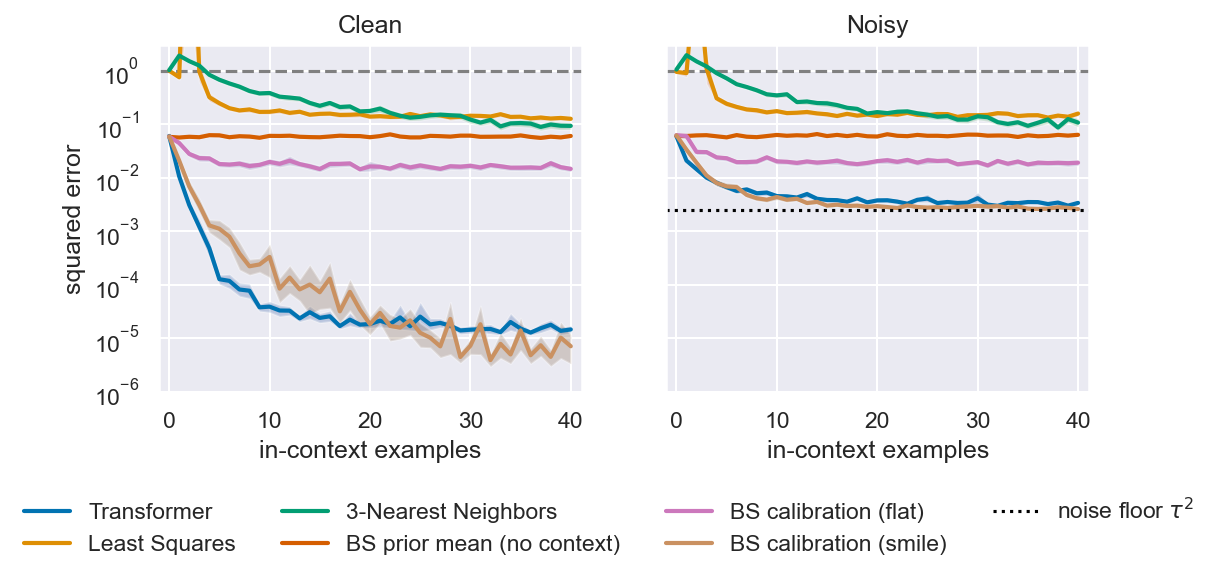
\includegraphics[width=0.9\linewidth]{figures/bs_smile/clean_vs_noisy.png}
\caption{\textbf{[YOUR caption: smile volatility; clean vs.\ noisy; gray dashed line =
error 1; dotted line = noise floor $\tau^2$]}}
\label{fig:bs-smile-noise}
\end{figure}

\paragraph{Scaled moneyness.}
On smile volatility (Figure~\ref{fig:bs-smile-scaling}), scaling by 2 leaves the
transformer's error at $k=40$ at $7.0\cdot10^{-4}$, still far below the prior mean (0.060),
but it stops improving after a few examples. Scaling by 3, it stays around $0.06$ for all
$k$ ($0.063$ at $k=40$), only slightly below the prior mean ($0.100$). Smile calibration
reaches at most $2.3\cdot10^{-6}$ in all cases, while misspecified flat calibration is
worse than the prior mean at scale 3 ($0.28$). On flat volatility the failure is even
clearer: at scale 3 the transformer's error ($0.082$) is above the prior mean ($0.073$) for
all $k$, i.e.\ it does worse than ignoring the examples, while calibration reaches
$6.3\cdot10^{-7}$.
\textbf{[What has the transformer learned, given that it works at $\times 2$ and fails at
$\times 3$? Why is calibration unaffected? Parallel to \cite{garg2022what}?]}

\begin{figure}[h]
\centering
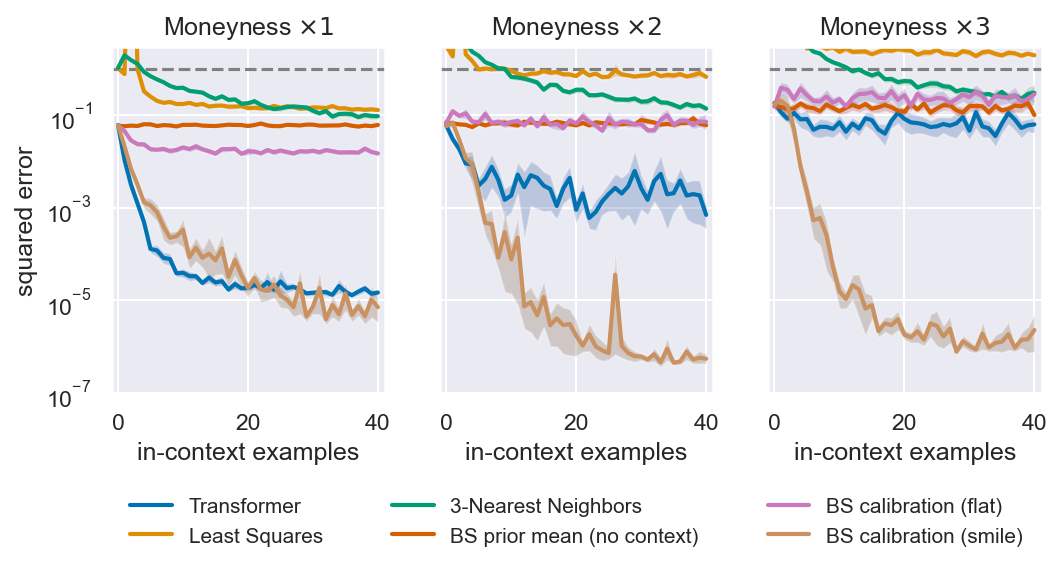
\includegraphics[width=0.9\linewidth]{figures/bs_smile/moneyness_scaling.png}
\caption{\textbf{[YOUR caption: smile volatility; moneyness scaled by 1, 2, 3 at test
time without retraining; gray dashed line = error 1]}}
\label{fig:bs-smile-scaling}
\end{figure}

\paragraph{Discussion and Limitations.}
Finding 1: the transformer falls below the prior mean after one example, and far
below flat calibration on smile volatility. What does each comparison rule out, i.e.\
which ``lazy'' strategy would each have caught?

Finding 2: on smile volatility the transformer beats calibration with the correct
model up to $k \approx 18$. What does the transformer have that calibration lacks, and why
does that advantage disappear at large $k$?

Finding 3: at moneyness $\times 3$ the transformer stops improving, while
calibration is unaffected. What does that say about what the transformer has learned:
the Black--Scholes formula itself, or something else? How does it compare with linear
regression under input scaling in \cite{garg2022what}?

Limitations: finish ``Because of this, we cannot claim that \ldots'' for
(i) one training run per task without a fixed seed;
(ii) no posterior-mean (Bayes-optimal) baseline;
(iii) the pricing formula and $r$ are the same in every prompt.
\newpage
{
\small
\bibliographystyle{plainnat}  % or IEEEtran
\bibliography{references}
}
\newpage
\section*{Statement on AI-use and contributions}

\subsection*{Tools}

Tool and version: Claude Code and Claude chat, models Sonnet 5.5 and Opus 5.5. 

Used for:

\begin{itemize}
    \item Literature review: "Summarize the discussion part of the paper"
    \item Paper/concept discussion: "The authors write that this \textit{suggests an effective learning algorithm}, but what does that mean?" and "Is this approach similar enough to the researchers' to be considered a variation or is it more of a new approach?" , 
    \item Codebase exploration: finding important functions and flows in the researchers codebase, using prompts like "where are the config parameters for the trained transformers being set"
    \item Boilerplate coding: "copy the format of the evals.py and adjust it generate figures using the provided plotting utilities in the codebase, but for the model we trained instead", 
    \item Architecture/Software adaptions: "write a script, using the config I gave you, to run the training on Modal instead of the implemented GPU setup". 
    \item Latex editing: "shorten this section so that it is 30\% shorter but that the content isn't modified?", "merge these two figures to subfigures", "any spelling or grammar errors?"
    \item Mathematics: checking notation consistency and correctness of derivations.
\end{itemize}

\subsection*{Declaration} 

We declare that:
every number, figure and table in this report was produced by running our own submitted code;
we understand every line of that code and can explain, modify and extend it without assistance;
the substance of this work — the implementation, the experiment, the analysis and the writing — is our own, and is not AI-generated work that we revised;
the account given above is complete and accurate.
this work was produced by our group alone; we have neither given nor received code, text, figures, results, or variation designs from any other group.
We understand that non-disclosure, or presenting AI-generated work as our own, is academic misconduct and will be reported.

\subsection*{Contributions}

Albin Jansson Sand, \texttt{albinjs}

Paper reading and discussion, participation in conceptual colearning, variation selection, writing mathematics and derivations, report writing, results discussions, presentation.

Harriet Källberg, \texttt{harrietk}

Paper reading and discussion, participation in conceptual colearning, variation selection, variation implementation, coding, training on Modal GPU, collecting results, matematics related to Black Scholes, report writing, report discussions, result discussions
\\
\\
\\
\\
\\
\\Albin Jansson Sand \hspace{10em} Harriet Källberg

Stockholm, 2026-10-08 \hspace{8em} Stockholm, 2026-10-08



\end{document}